\documentclass[justified]{tufte-handout}
\usepackage{amsmath}
\usepackage{booktabs}
\usepackage{graphicx}
\graphicspath{{figures/}}

\title{Stereo Disparity and Relative Depth on OpenCV Aloe}
\author{Xuanye Xu, Student IDs: 24020036071 / H00490299}
\date{Robotics Integration Project I \quad 25 September 2026}

\begin{document}
\maketitle

\begin{abstract}
This experiment computes stereo disparity and a relative-depth proxy for
OpenCV's Aloe image pair. Both images were reduced to \(641\times555\)
pixels and processed with StereoSGBM. The default result contains valid
positive disparity at 70.5\% of pixels. Regions on the plant and pot have
larger median disparity than the background, as expected for nearer
surfaces. The data used here do not include a verified metric baseline
or focal length; the resulting depth values are therefore not distances
in meters.
\end{abstract}

\section{Aim and data}

The aim was to produce disparity, inspect its failures, and demonstrate
the inverse relationship between disparity and depth. The inputs were
\texttt{aloeL.jpg} and \texttt{aloeR.jpg} from OpenCV's
\texttt{samples/data} collection. Both originals are
\(1282\times1110\) pixels; the program scales each dimension by
one half before matching. The provided pair is treated as rectified
for horizontal matching \citep{opencv_sample}. Horizontal guide lines in
the recorded input pair support visual inspection of the alignment.

\begin{figure*}[ht]
  \centering
  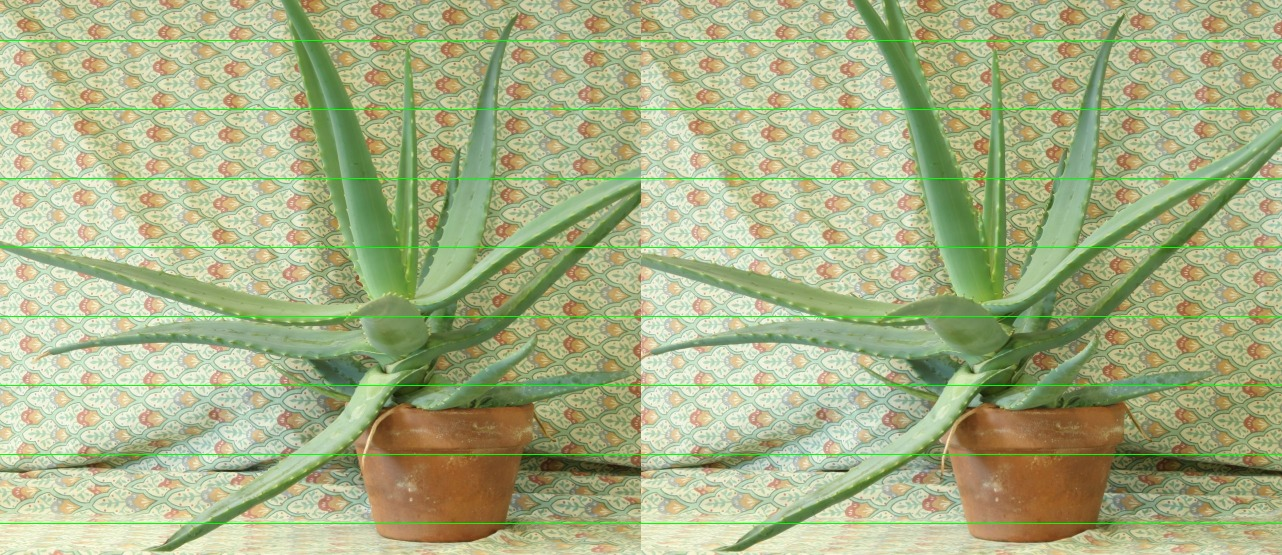
\includegraphics[width=0.82\linewidth]{stereo_pair.jpg}
  \caption{The left and right Aloe inputs after resizing. Horizontal guide
  lines show the scanlines used for visual alignment checks.}
\end{figure*}

\section{Method}

Stereo rectification maps corresponding epipolar lines to horizontal
scanlines. The rectification paper by Fusiello et al. \citep{fusiello2000} explains this
geometric step; the present code starts from the already aligned sample
pair and performs matching. A grayscale StereoSGBM matcher used
\(\texttt{minDisparity}=0\), \(\texttt{numDisparities}=128\),
\(\texttt{blockSize}=5\), \(P_1=200\), \(P_2=800\),
\(\texttt{uniquenessRatio}=10\), and a 100-pixel speckle window.
OpenCV's signed fixed-point output was divided by 16 to obtain
pixel disparity \(d=u_L-u_R\). Nonpositive and nonfinite values were
excluded.

For ideal horizontally rectified cameras with equal horizontal
principal points, depth would satisfy \(Z=fB/d\). The OpenCV Aloe
example \citep{opencv_sample} \emph{guesses} \(f=0.8w\), where \(w=641\) pixels after
resizing. Following that illustration, the program used
\(f=512.8\) px and \(B=1\) arbitrary baseline unit:
\begin{equation}
  Z_{\mathrm{proxy}}=\frac{512.8}{d}.
\end{equation}
This proxy preserves the near/far ordering for positive disparities.
Its numerical values cannot be converted to meters from the available
inputs. The estimated focal length and baseline assumption are recorded
in \texttt{summary.json}.

\begin{figure*}[ht]
  \centering
  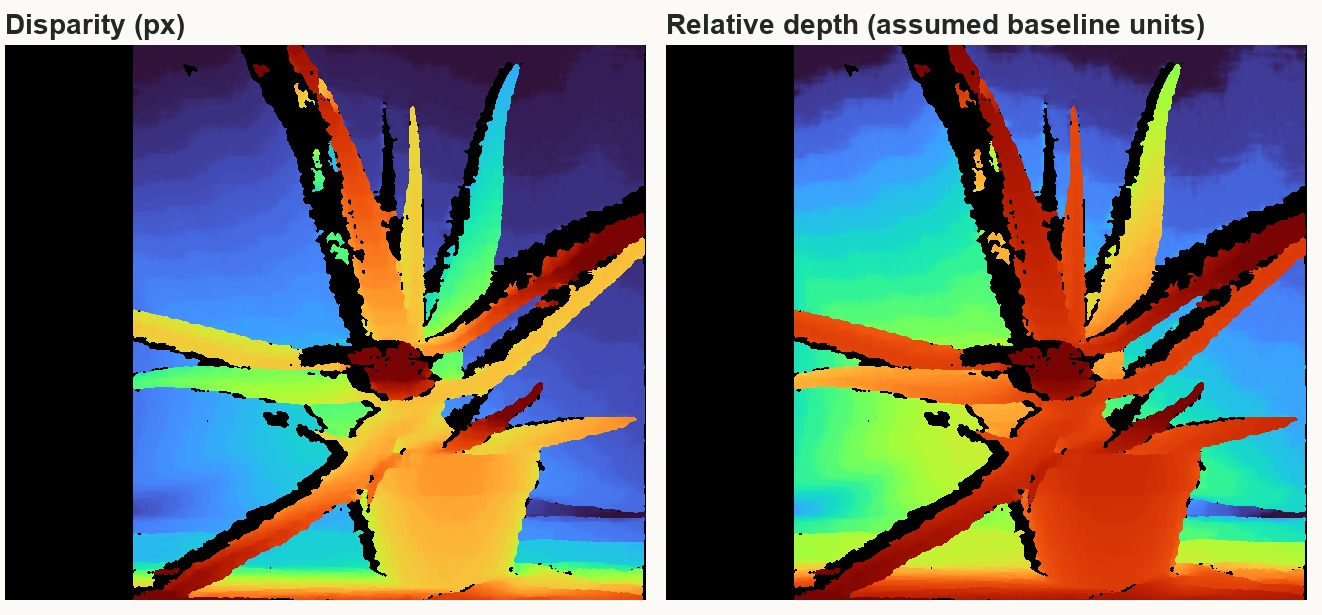
\includegraphics[width=0.88\linewidth]{stereo_maps.jpg}
  \caption{Computed disparity and illustrative relative depth. Black
  denotes excluded pixels. Colors are independently mapped over the
  2nd--98th percentile range for visibility, so numeric comparisons
  must use the saved arrays rather than image colors.}
\end{figure*}

\section{Results}

Of \(641\times555=355{,}755\) pixels, \(70.5\%\) have valid positive
disparity. Across those pixels, the 5th, median, and 95th disparity
percentiles are \(23.875\), \(32.063\), and \(65.250\) px.
The corresponding \emph{distribution} of relative-depth values has
5th, median, and 95th percentiles of \(7.859\), \(15.994\), and
\(21.479\) assumed baseline units. These distributions are reported
separately; percentile positions reverse under the inverse mapping.

Three fixed regions were sampled: wallpaper background (B), central
leaf/core (L), and pot (P). Their locations are marked in the retained
figure asset.

\begin{table}[ht]
  \centering
  \begin{tabular}{lrrr}
  \toprule
  Region & Valid & Median \(d\) & Median \(Z_{\rm proxy}\)\\
         & (\%) & (px) & (baseline units)\\
  \midrule
  Background (B) & 52.0 & 25.69 & 19.96\\
  Leaf/core (L)  & 78.1 & 58.00 & 8.84\\
  Pot (P)        & 99.5 & 56.00 & 9.16\\
  \bottomrule
  \end{tabular}
  \caption{Descriptive values over valid pixels inside the marked
  rectangles. They are not ground-truth accuracy measurements.}
\end{table}

Increasing the matching block size from 5 to 9 changed the valid-pixel
fraction from \(70.5\%\) to \(70.8\%\). On pixels valid in both runs,
the median absolute disparity difference was \(0.062\) px.
This small aggregate change does not establish accuracy, especially
at object edges and occlusions.

\section{Interpretation and limits}

The plant and pot show larger disparities than the patterned background,
consistent with their closer position. Missing values occur near image
borders, thin leaves, occlusions, and difficult texture. Repeated
wallpaper motifs can also yield incorrect correspondences. No
ground-truth disparity, measured baseline, or camera calibration was
available for this pair. Consequently the experiment demonstrates
relative depth only; a metric depth map would require calibrated stereo
parameters and a matching rectification model.

\section{Reproduction}

The run used Python 3.9.23, NumPy 2.0.2, and OpenCV 4.12.0.
From the repository root:
\begin{quote}\small\ttfamily
python3.9 lab0/code/stereo\_depth.py\\
\quad --sample --scale 0.5
\end{quote}
The raw disparity, valid mask, relative-depth array, images, and run
parameters are under \path{lab0/results/stereo/}. A second run set the
block size to 9.

\enlargethispage{5\baselineskip}
\bibliographystyle{plainnat}
\bibliography{lab0_references}

\end{document}
